\documentclass{beamer}
\usepackage{amsmath}
\usepackage[english]{babel} %set language; note: after changing this, you need to delete all auxiliary files to recompile
\usepackage[utf8]{inputenc} %define file encoding; latin1 is the other often used option
\usepackage{csquotes} % provides context sensitive quotation facilities
\usepackage{graphicx} %allows for inserting figures
\usepackage{booktabs} % for table formatting without vertical lines
\usepackage{textcomp} % allow for example using the Euro sign with \texteuro
\usepackage{stackengine}
\usepackage{wasysym}
\usepackage{tikzsymbols}
\usepackage{textcomp}
\newcommand{\bubblethis}[2]{
        \tikz[remember picture,baseline]{\node[anchor=base,inner sep=0,outer sep=0]%
        (#1) {\underline{#1}};\node[overlay,cloud callout,callout relative pointer={(0.2cm,-0.7cm)},%
        aspect=2.5,fill=yellow!90] at ($(#1.north)+(-0.5cm,1.6cm)$) {#2};}%
    }%
\tikzset{face/.style={shape=circle,minimum size=4ex,shading=radial,outer sep=0pt,
        inner color=white!50!yellow,outer color= yellow!70!orange}}
%% Some commands to make the code easier
\newcommand{\emoticon}[1][]{%
  \node[face,#1] (emoticon) {};
  %% The eyes are fixed.
  \draw[fill=white] (-1ex,0ex) ..controls (-0.5ex,0.2ex)and(0.5ex,0.2ex)..
        (1ex,0.0ex) ..controls ( 1.5ex,1.5ex)and( 0.2ex,1.7ex)..
        (0ex,0.4ex) ..controls (-0.2ex,1.7ex)and(-1.5ex,1.5ex)..
        (-1ex,0ex)--cycle;}
\newcommand{\pupils}{
  %% standard pupils
  \fill[shift={(0.5ex,0.5ex)},rotate=80] 
       (0,0) ellipse (0.3ex and 0.15ex);
  \fill[shift={(-0.5ex,0.5ex)},rotate=100] 
       (0,0) ellipse (0.3ex and 0.15ex);}

\newcommand{\emoticonname}[1]{
  \node[below=1ex of emoticon,font=\footnotesize,
        minimum width=4cm]{#1};}
\usepackage{scalerel}
\usetikzlibrary{positioning}
\usepackage{xcolor,amssymb}
\newcommand\dangersignb[1][2ex]{%
  \scaleto{\stackengine{0.3pt}{\scalebox{1.1}[.9]{%
  \color{red}$\blacktriangle$}}{\tiny\bfseries !}{O}{c}{F}{F}{L}}{#1}%
}
\newcommand\dangersignw[1][2ex]{%
  \scaleto{\stackengine{0.3pt}{\scalebox{1.1}[.9]{%
  \color{red}$\blacktriangle$}}{\color{white}\tiny\bfseries !}{O}{c}{F}{F}{L}}{#1}%
}
\usepackage{fontawesome} % Social Icons
\usepackage{epstopdf} % allow embedding eps-figures
\usepackage{tikz} % allows drawing figures
\usepackage{amsmath,amssymb,amsthm} %advanced math facilities
\usepackage{lmodern} %uses font that support italic and bold at the same time
\usepackage{hyperref}
\usepackage{tikz}
\hypersetup{
    colorlinks=true,
    linkcolor=blue,
    filecolor=magenta,      
    urlcolor=blue,
}
\usepackage{tcolorbox}
%add citation management using BibLaTeX
\usepackage[citestyle=authoryear-comp, %define style for citations
    bibstyle=authoryear-comp, %define style for bibliography
    maxbibnames=10, %maximum number of authors displayed in bibliography
    minbibnames=1, %minimum number of authors displayed in bibliography
    maxcitenames=3, %maximum number of authors displayed in citations before using et al.
    minnames=1, %maximum number of authors displayed in citations before using et al.
    datezeros=false, % do not print dates with leading zeros
    date=long, %use long formats for dates
    isbn=false,% show no ISBNs in bibliography (applies only if not a mandatory field)
    url=false,% show no urls in bibliography (applies only if not a mandatory field)
    doi=false, % show no dois in bibliography (applies only if not a mandatory field)
    eprint=false, %show no eprint-field in bibliography (applies only if not a mandatory field)
    backend=biber %use biber as the backend; backend=bibtex is less powerful, but easier to install
    ]{biblatex}
\addbibresource{../mybibfile.bib} %define bib-file located one folder higher


\usefonttheme[onlymath]{serif} %set math font to serif ones

\definecolor{beamerblue}{rgb}{0.2,0.2,0.7} %define beamerblue color for later use

%%% defines highlight command to set text blue
\newcommand{\highlight}[1]{{\color{blue}{#1}}}


%%%%%%% commands defining backup slides so that frame numbering is correct

\newcommand{\backupbegin}{
   \newcounter{framenumberappendix}
   \setcounter{framenumberappendix}{\value{framenumber}}
}
\newcommand{\backupend}{
   \addtocounter{framenumberappendix}{-\value{framenumber}}
   \addtocounter{framenumber}{\value{framenumberappendix}}
}

%%%% end of defining backup slides

%Specify figure caption, see also http://tex.stackexchange.com/questions/155738/caption-package-not-working-with-beamer
\setbeamertemplate{caption}{\insertcaption} %redefines caption to remove label "Figure".
%\setbeamerfont{caption}{size=\scriptsize,shape=\itshape,series=\bfseries} %sets figure  caption bold and italic and makes it smaller


\usetheme{Boadilla}

%set options of hyperref package
\hypersetup{
    bookmarksnumbered=true, %put section numbers in bookmarks
    naturalnames=true, %use LATEX-computed names for links
    citebordercolor={1 1 1}, %color of border around cites, here: white, i.e. invisible
    linkbordercolor={1 1 1}, %color of border around links, here: white, i.e. invisible
    colorlinks=true, %color links
    anchorcolor=black, %set color of anchors
    linkcolor=beamerblue, %set link color to beamer blue
    citecolor=blue, %set cite color to beamer blue
    pdfpagemode=UseThumbs, %set default mode of PDF display
    breaklinks=true, %break long links
    pdfstartpage=1 %start at first page
    }


% --------------------
% Overall information
% --------------------
\title[Economía I]{Economía I \vspace{4mm}
\\ Magistral 18: Intro a la macroeconomía }
\date{}
\author[Ertola Navajas y Fariña]{Ertola Navajas y Fariña}
\vspace{0.4cm}
\institute[]{Universidad de San Andrés} 

\begin{document}

\begin{frame}
\titlepage
\centering


\includegraphics[scale=0.2]{Slides Principios de Economia/Figures/logoUDESA.jpg} 
\end{frame}



\begin{frame}
\frametitle{La micro y la macro}
\begin{itemize}
        \item Disciplinas dentro de economía
        \vspace{2mm}
        \begin{itemize}
        \item Hasta ahora hemos visto cosas que se suelen asociar con la microeconomía \\
        - ¿Cómo los agentes interactúan entre sí y toman decisiones?
        \vspace{2mm}
        \item Ahora nos metemos en temas de macroeconómica \\
        - ¿Cómo funciona la economía en su conjunto, donde cambios económicos afectan a los agentes en forma simultánea?
        \end{itemize}
\end{itemize}
\end{frame}


\begin{frame}{Macroeconomía}
   \begin{itemize}
       \item La macroeconomía tiene que ver con los resultados "agregados" de la economía \vspace{1mm}
       \item Vamos a ver qué son y cómo medir los agregados económicos: la actividad, los precios, el desempleo, etc. \vspace{1mm}
       \item También vamos a estudiar los ciclos económicos: porque el crecimiento viene acompañado de booms y recesiones \vspace{1mm}
       \item Finalmente, vamos a discutir políticas: ¿qué variables afectan la política fiscal y monetaria? 
   \end{itemize} 
\end{frame}

\begin{frame}
\frametitle{Evaluando toda la economía}
\begin{itemize}
        \item Para evaluar la forma en que una persona está en términos económicos uno suele mirar sus ingresos \vspace{1mm}
        \item Para una economía hacemos lo mismo, pero una economía es un sistema en el que diversos agentes interactúan \vspace{1mm}
        \begin{itemize}
            \item Hogares
            \item Empresas
            \item Instituciones financieras
            \item Gobierno
            \item Sector externo
        \end{itemize}
\end{itemize}
\end{frame}

\begin{frame}{Flujo circular de la riqueza}
    \begin{figure} [H]
\centering
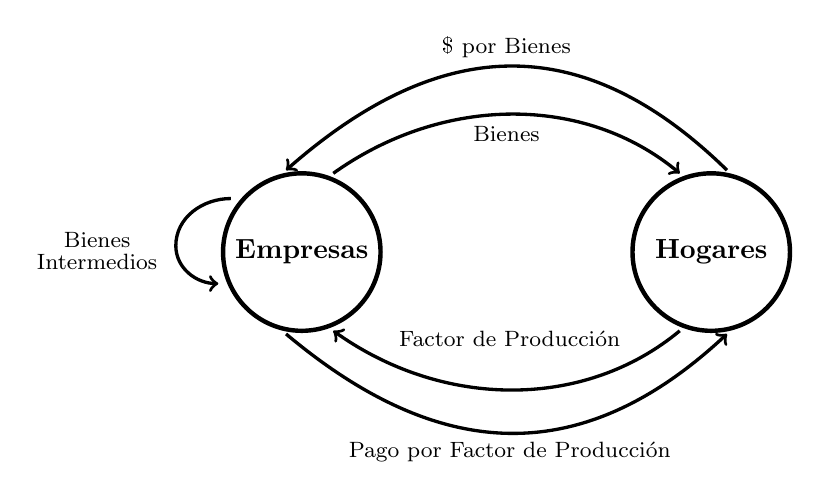
\begin{tikzpicture}[scale=0.4]
\draw[ultra thick](2,0) circle [radius =2.5];
\node[] at (2,0) { \textbf{Empresas}};
\draw[ultra thick](15,0) circle [radius =2.5];
\node[] at (15,0) {\textbf{Hogares} };
\draw [very thick, ->] (-0.25, 1.7) to [out=-180, in=90] (-2, 0.2) to [out=-90, in=180] (-0.65, -1);
\node[] at (-4.5,0.4) {\footnotesize  Bienes};
\node[] at (-4.5,-0.3) {\footnotesize  Intermedios};
\draw[very thick, ->] (3,2.5).. controls (6.5,5) and (11,5) .. (14,2.5);
\draw[very thick, <-] (1.5,2.6).. controls (6.5,7) and (11,7) .. (15.5,2.6);
\node[] at (8.5,3.75) {\footnotesize  Bienes};
\node[] at (8.5,6.5) {\footnotesize  \$ por Bienes};
\draw[very thick, <-] (3,-2.5).. controls (6.5,-5) and (11,-5) .. (14,-2.5);
\draw[very thick, ->] (1.5,-2.6).. controls (6.5,-6.8) and (11,-6.8) .. (15.5,-2.6);
\node[] at (8.6,-2.75) {\footnotesize  Factor de Producción};
\node[] at (8.6,-6.35) {\footnotesize Pago por Factor de Producción};
\end{tikzpicture}
\label{fig:25.1}
\end{figure} 

\end{frame}


\begin{frame}{}
\centering\huge\textbf{Midiendo la producción} 
\vspace{2mm}
\hrule
\end{frame}

\begin{frame}{Definiendo el PBI}
\begin{itemize}
   \item El Producto Bruto Interno (PBI) es una medida del producto total de una economía \vspace{1mm}
   \item ¡Noten que la suma de los bienes es igual a la suma de los ingresos! \vspace{1mm}
   \item Por eso a veces nos referimos al PBI como ingreso nacional
   \end{itemize}
\end{frame}

\begin{frame}
\frametitle{El PBI}
\begin{itemize}
        \item Mirándolo en términos de gasto, el PBI es el valor de mercado de todos bienes finales y servicios producidos en una economía durante un período de tiempo determinado \vspace{1mm}
        \begin{itemize}
            \item ``Valor de mercado'' \\ 
            - Utiliza los precios que la gente está dispuesta a pagar \vspace{1mm}
            \item ``todos los bienes finales y servicios'' \\
            - Bienes tangibles y servicios intangibles \\
            - No se cuenta bienes intermedios \\
            - Todo lo producido en la economía\\ \vspace{1mm}
            \item ``en una economía, durante un período determinado'' \\
            - Producción dentro de los límites geográficos \\
            - Un flujo de un intervalo de tiempo \\ 
        \end{itemize}
\end{itemize}
\end{frame}

\begin{frame}{Midiendo el PBI}
    \begin{itemize}
        \item Tenemos tres maneras de medirlo \vspace{1mm}
       \begin{itemize}
           \item Por el gasto (valor de los bienes finales consumidos) \vspace{1mm}
           \item Por los ingresos (suma de los ingresos recibidos) \vspace{1mm}
           \item La producción (total producido por la industria) \\
            - Aquí se mide el valor agregado en la producción de cada industria
       \end{itemize}
    \end{itemize}
\end{frame}

\begin{frame}{Un ejemplo de cómo medir el PBI}
    \begin{figure} [H]   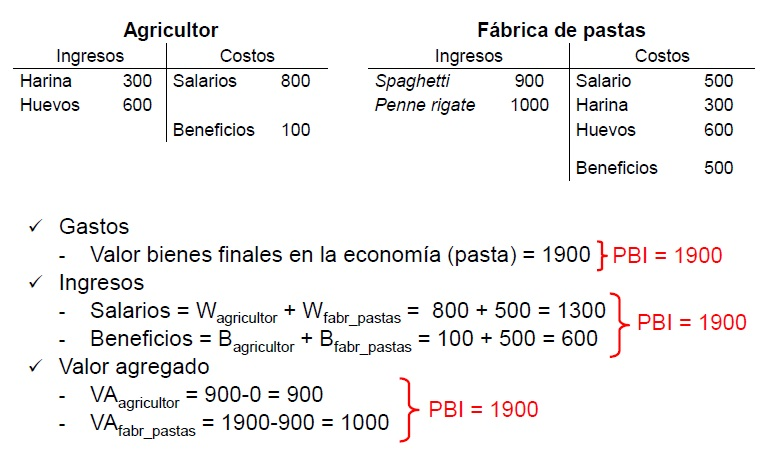
\includegraphics[scale=0.55]{Slides Principios de Economia/Figures/C16.2.jpg}
\label{fig:25.2}
\end{figure}
\end{frame}

\begin{frame}{La medición no es sencilla....  ¿Cuánto es el dinero que movilizan los clubes del fútbol argentino?.}

\end{frame}


\begin{frame}{¿Cuánto es el dinero que movilizan los clubes del fútbol argentino?.}
    \begin{figure} [H]   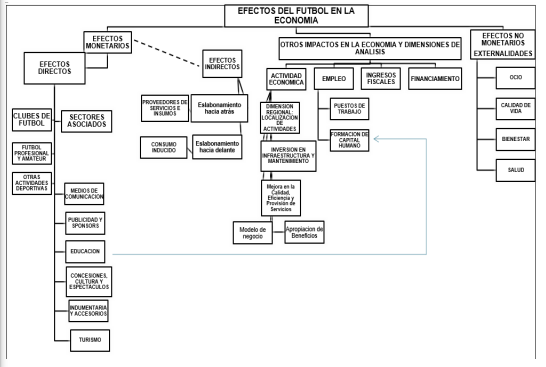
\includegraphics[scale=0.7]{Slides Principios de Economia/Figures/PBIFutbol.png}
\label{fig:25.2}
\end{figure}
\end{frame}

\begin{frame}{¿Cuánto es el dinero que movilizan los clubes del fútbol argentino?.}
    \begin{figure} [H]   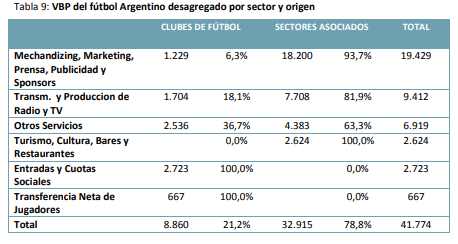
\includegraphics[scale=0.75]{Slides Principios de Economia/Figures/PBIFutbolII.png}
\label{fig:25.2}
\end{figure}
\end{frame}

\begin{frame}
\frametitle{Otros elementos importantes}
\begin{itemize}
        \item ¿Cómo incorporamos el sector externo?
        \begin{itemize}
            \item Parte de la producción extranjera es el consumo interno (importaciones) y parte de la producción nacional es consumo extranjero (exportaciones) \\ 
            - El PBI incluye valor agregado, ingresos de, o consumo de producción nacional \\
            - Incluimos exportaciones y excluimos importaciones
            \end{itemize} \vspace{1mm}
        \item ¿Cómo incorporamos al gobierno?
        \begin{itemize}
            \item Se lo trata básicamente como otro productor \\
            - Servicios públicos son “comprados” con impuestos \\
            - El costo de producción captura la valor agregado
            \end{itemize}
\end{itemize}
\end{frame}


\begin{frame}
\frametitle{Sector externo}
\begin{figure} [H]
\centering
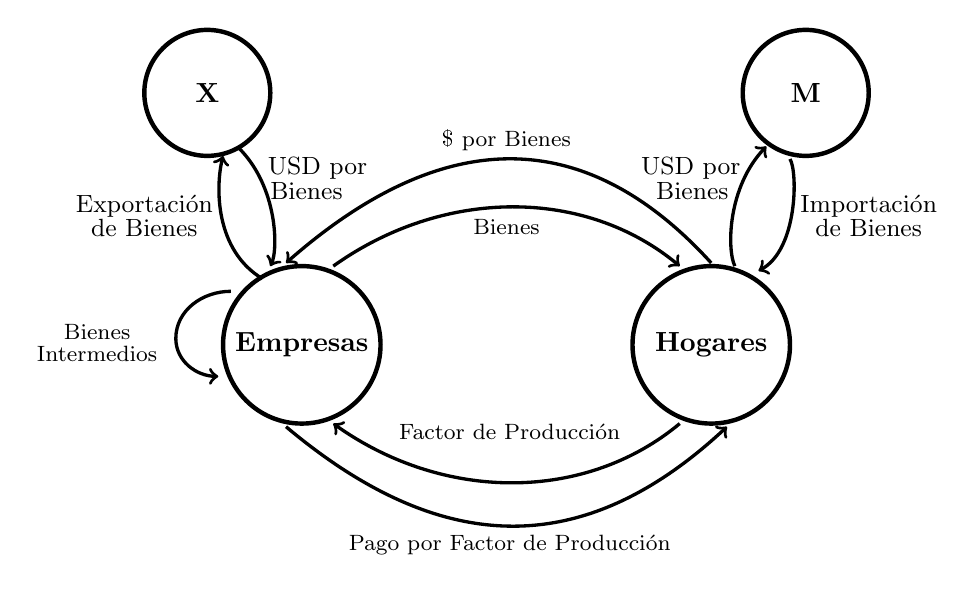
\begin{tikzpicture}[scale=0.4]
\draw[ultra thick](2,0) circle [radius =2.5];
\node[] at (2,0) { \textbf{Empresas}};
\draw[ultra thick](15,0) circle [radius =2.5];
\node[] at (15,0) { \textbf{Hogares} };
\draw[ultra thick](18,8) circle [radius =2];
\node[] at (18,8) { \textbf{M}};
\draw[ultra thick](-1,8) circle [radius =2];
\node[] at (-1,8) {\textbf{X}};
\draw [very thick, ->] (-0.25, 1.7) to [out=-180, in=90] (-2, 0.2) to [out=-90, in=180] (-0.65, -1);
\node[] at (-4.5,0.4) { \footnotesize Bienes};
\node[] at (-4.5,-0.3) {\footnotesize  Intermedios};
\draw[very thick, ->] (3,2.5).. controls (6.5,5) and (11,5) .. (14,2.5);
\draw[very thick, <-] (1.5,2.6).. controls (6.5,7) and (11,7) .. (15,2.6);
\node[] at (8.5,3.75) {\footnotesize  Bienes};
\node[] at (8.5,6.5) {\footnotesize  \$ por Bienes};
\draw[very thick, <-] (3,-2.5).. controls (6.5,-5) and (11,-5) .. (14,-2.5);
\draw[very thick, ->] (1.5,-2.6).. controls (6.5,-6.8) and (11,-6.8) .. (15.5,-2.6);
\node[] at (8.6,-2.75) { \footnotesize Factor de Producción};
\node[] at (8.6,-6.35) {\footnotesize Pago por Factor de Producción};
\draw[very thick, <-] (1,2.5).. controls (1.25,3) and (1.25,5) .. (0,6.25);
\draw[very thick, ->] (0.75,2.1).. controls (-0.75,3) and (-0.75,5) .. (-0.5,6);
\draw[very thick, <-] (16.5,2.35).. controls (17.75,3) and (17.75,5.5) .. (17.5,5.9);
\draw[very thick, ->] (15.75,2.5).. controls (15.5,3) and (15.5,5) .. (16.75,6.3);
\node[] at (-3,4.4) {\small  Exportación};
\node[] at (-3,3.7) {\small  de Bienes};
\node[] at (2.5,5.6) {\small  USD por};
\node[] at (2.15,4.9) {\small  Bienes};
\node[] at (20,4.4) {\small  Importación};
\node[] at (20,3.7) {\small  de Bienes};
\node[] at (14.35,5.6) {\small  USD por};
\node[] at (14.4,4.9) {\small  Bienes};
\end{tikzpicture}
\end{figure} 
\end{frame}

\begin{frame}{Temas en la medición del PBI}
    \begin{itemize}
        \item Ventas de bienes ya producidos no van (ejemplo: venta de una casa)
        \item Transferencias de ingresos no van (ejemplo: jubilaciones) 
        \item ¿Planes sociales? Depende! (ejemplo: AUH vs Plan Jefes y Jefas de Hogares)
        \item Se incorpora una estimación de la economía informal
        \item Los bienes y servicios producidos por el Estado tambien deben incorporarse
        \begin{itemize}
            \item Pero al ser difícil asignar un valor de mercado a estos bienes y servicios, se los agrega al costo de producción
        \end{itemize}
        \item Algunas discusiones: productos de internet y ajustes por calidad
    \end{itemize}
\end{frame}

\begin{frame}{Buscando los datos}
    \begin{itemize}
        \item Cada país tiene su agencia de estadísticas \vspace{1mm}
        \item En Argentina es el \href{https://www.indec.gob.ar/}{INDEC} \vspace{1mm}
        \item Pueden ver también \href{https://www.alphacast.io/}{Alphacast} \vspace{1mm}
        \item Para bases de datos homogéneas:  \href{https://data.imf.org/?sk=4c514d48-b6ba-49ed-8ab9-52b0c1a0179b}{FMI}\vspace{1mm}
        \item Para perspectivas futuras: \href{https://www.imf.org/en/Publications/WEO}{WEO}\vspace{1mm} 
        \item Para otra visión: FRED     
    \end{itemize}
\end{frame}


\begin{frame}
\frametitle{Argentina y el crecimiento mundial}
\begin{center}
\href{https://www.gapminder.org/tools/#$model$markers$line$data$filter$dimensions$country$country$/$in@=usa&=chn&=arg&=bra&=nzl&=can&=aus;;;;;;&encoding$selected$data$filter$markers@=aus&=arg;;;;;;;;&chart-type=linechart&url=v1} {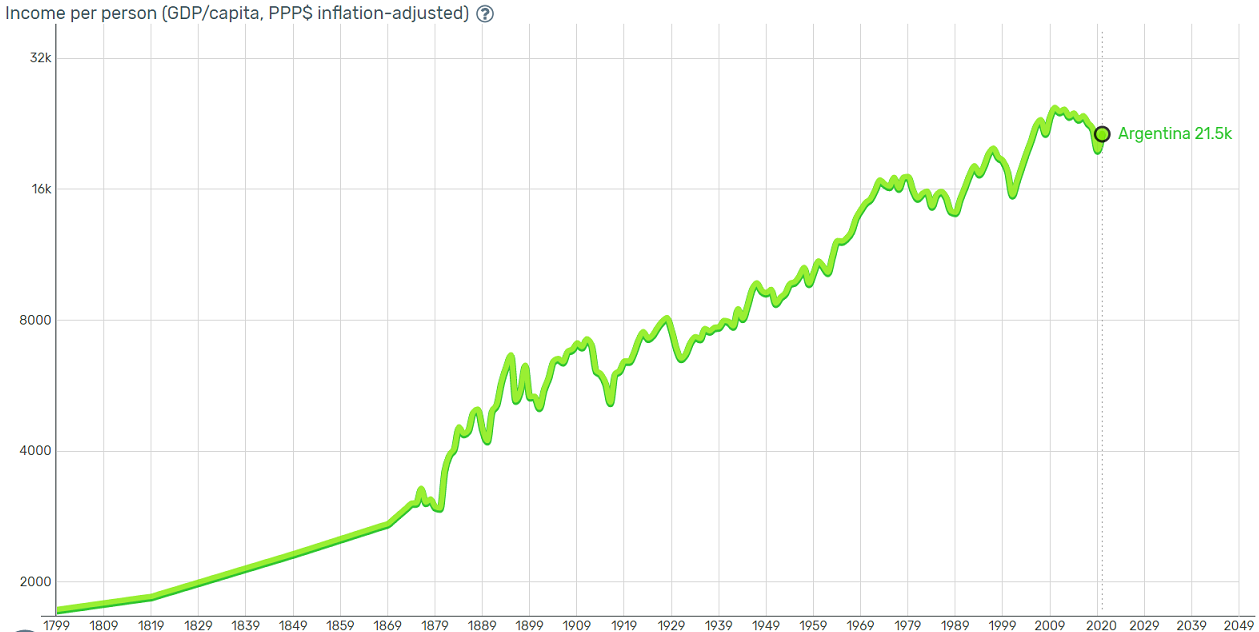
\includegraphics[width=0.9\textwidth]{Slides Principios de Economia/Figures/gdparg.png}}
\end{center}
Fuente: Gapminder
\end{frame}

\begin{frame}{}
\centering\huge\textbf{PBI y PBN} 
\vspace{2mm}
\hrule
\end{frame}

\begin{frame}{PBI y PBN}
    \begin{itemize}
        \item El Producto Bruto Nacional (PBN) es el PBI ajustado por el retorno a los factores externos
    \end{itemize}
\begin{figure} [h!]
    \centering
    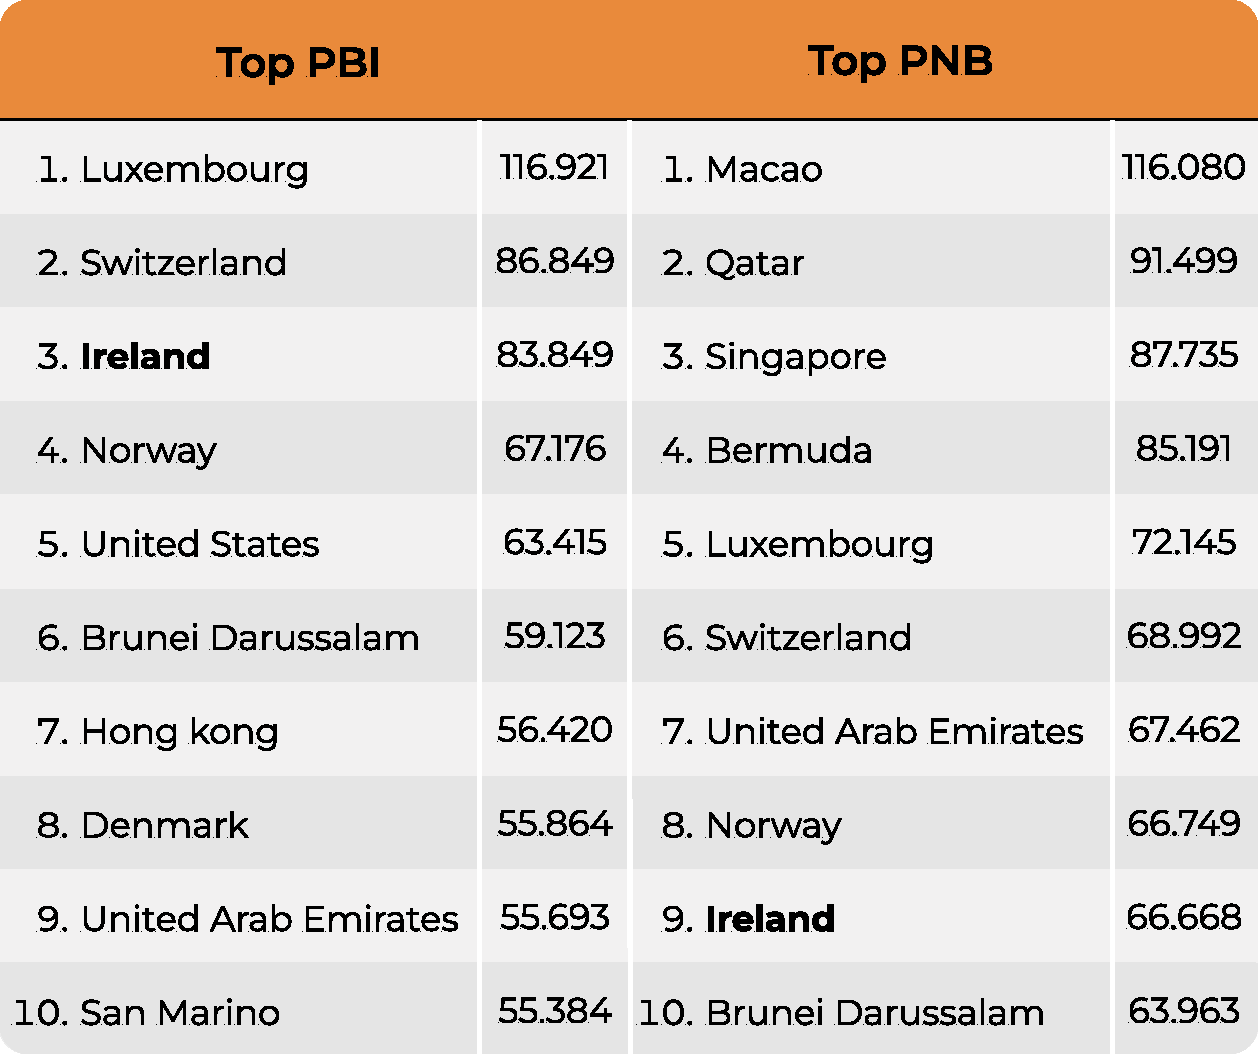
\includegraphics[width=0.65\textwidth]{Slides Principios de Economia/Figures/T 29.1.pdf}
\end{figure}
\end{frame}

\begin{frame}{Un caso extraordinario }
    
\begin{figure} [H]
\centering
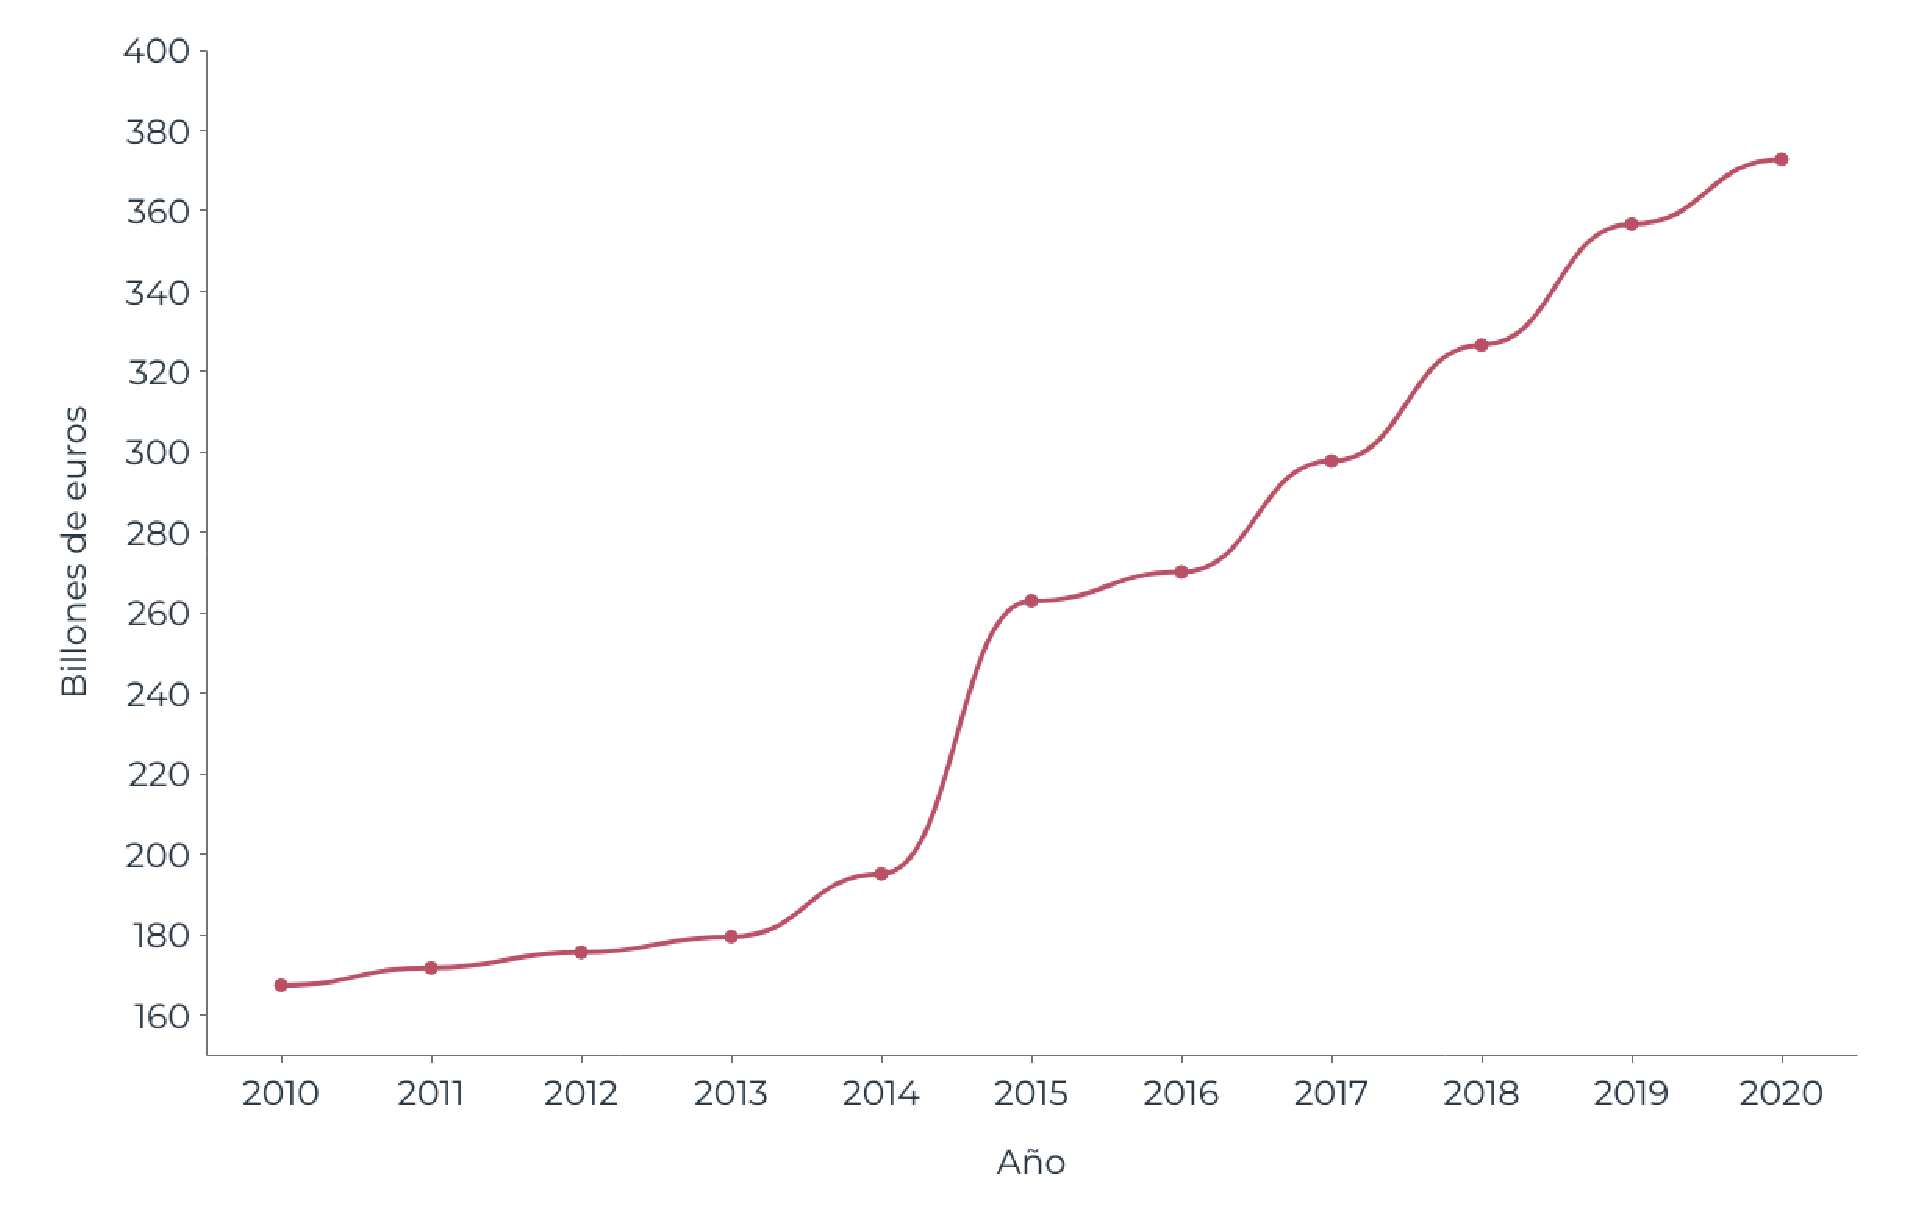
\includegraphics[width=0.9\textwidth]{Slides Principios de Economia/Figures/29.4.pdf}
\caption{PBI Irlanda a precios constantes}
\label{fig:G1}
\end{figure} 
\end{frame}

%\begin{frame}{Graficando el PBI de EEUU a largo plazo}
%    \begin{figure} [H]   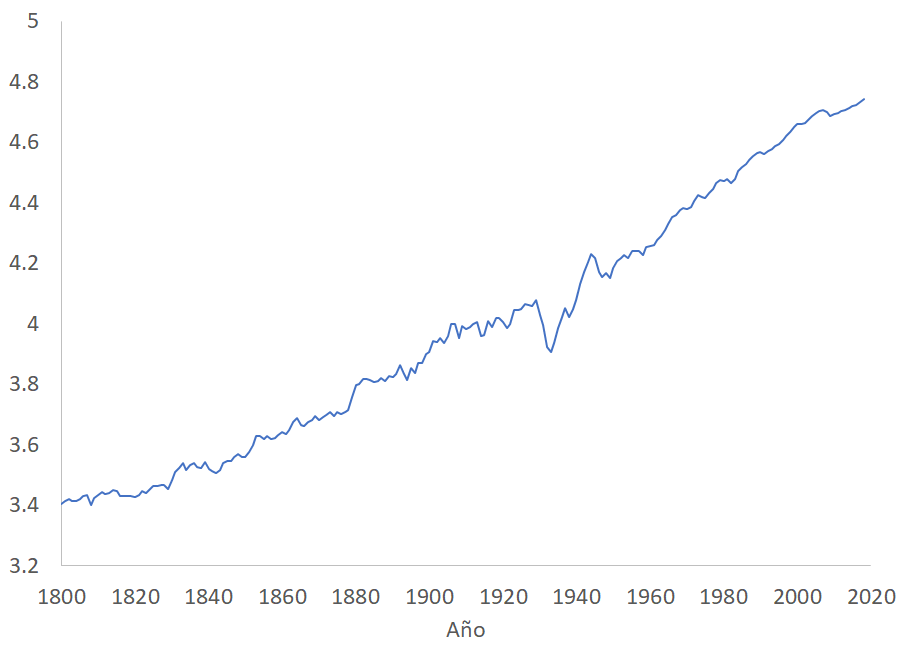
\includegraphics[scale=1]{Slides Principios de Economia/Figures/G2.png}
%\end{figure}
%\end{frame}

%\begin{frame}{Ajustando con logs}
%    \begin{center}
%\begin{figure}[H]
%\renewcommand{\figurename}{Figure}
%\begin{center}
%    \begin{minipage}[b]{0.35\textwidth}
%        \begin{center}
%\begin{tikzpicture}[scale=0.4]
%\draw[very thick,<->] (0,11) node[left]{$f$}--(0,0)--(11,0) node[below]{$x$};
%\draw[semithick] (0,1).. controls (3,1) and (8, 1.1) .. (8.5, 8) node [right]{\footnotesize $Ae^{\lambda x}$};
%\end{tikzpicture}
%\end{center}
%     \end{minipage}
  %  \hfill
    %\begin{minipage}[b]{0.4\textwidth}
    %\begin{center}
%\begin{tikzpicture}[scale=0.35]
%\draw[very thick,<->] (0,11) node[left]{$f$}--(0,0)--(11,0) node[below]{$x$};
%\draw[semithick] (0,2)--(9, 7) node [right]{\footnotesize $log(Ae^{\lambda x})$};
%\draw[semithick, gray] (1,2.5)--(2,2.5)--(2,3.1);
%\node[] at (1.6,2) {\scriptsize $\lambda$};
%\node[left] at (0,2) {\footnotesize $log(A)$};
%\node[] at (11,6) {\footnotesize $=$};
%\node[] at (10.75,5.25) {\footnotesize $log(A)+\lambda x$};
%\end{tikzpicture}
%\end{center}
%    \end{minipage}
%\end{center}
%\end{figure}
%\end{center} 
%\end{frame}

%\begin{frame}{Re-graficando el PBI de EEUU a largo plazo en logs}
%   \begin{figure} [H]   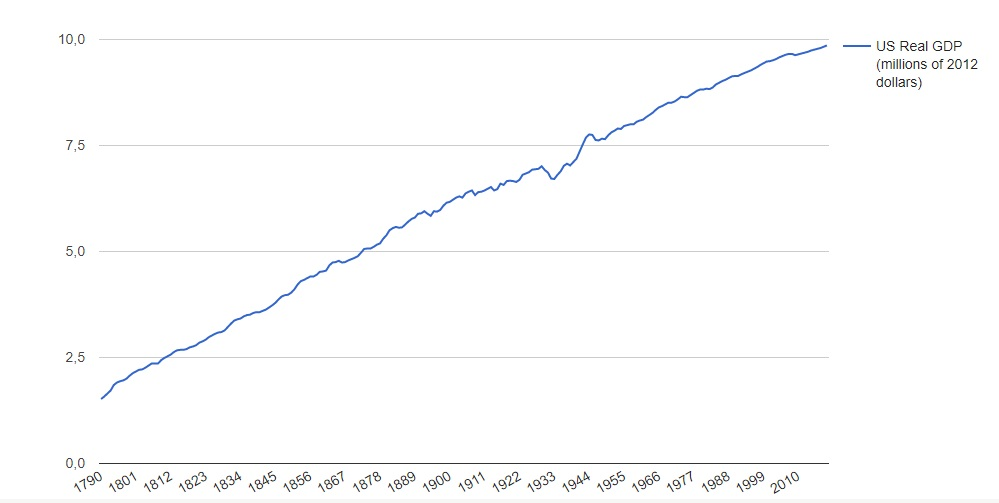
\includegraphics[scale=0.45]{Slides Principios de Economia/Figures/C16.4.jpg}
%\end{figure}
%Fuente: \href{https://www.measuringworth.com/graphs/}{www.measuringworth.com}
%\end{frame}


\begin{frame}{}
\centering\huge\textbf{PBI Real y nominal} 
\vspace{2mm}
\hrule
\end{frame}

\begin{frame}
\frametitle{PBI real y nominal}
\begin{itemize}
        \item Pensemos en la definición del PBI nominal
        \\ \vspace{1mm}
        \begin{center} \small{
            $PBI_{nominal}^{\text{año t}}=p_{1}^{\text{año t}}q_{1}^{\text{año t}}+p_{2}^{\text{año t}}q_{2}^{\text{año t}}+...+p_{N}^{\text{año t}}q_{N}^{\text{año t}}$}
        \end{center}
        \\ \vspace{1mm}
        \begin{itemize}
            \item Si el gasto se eleva de un año al siguiente: \\
            - ¿Se está produciendo más en la economía? \\
            - ¿Los bienes y servicios se venden a precios más altos?
            \end{itemize} \vspace{1mm}
        \item El PBI real
        \begin{itemize}
            \item ¿Cuál sería el valor de los bienes y servicios producidos en un año si los valoramos a precios que prevalecieron en algún año específico? \\
            - ¿Qué es una buen año ‘base’?
            \end{itemize} \vspace{1mm}
        \item ¿Por qué es importante la diferencia entre nominal y real? \href{https://www.gapminder.org/tools/#$model$markers$line$data$filter$dimensions$country$country$/$in@=arg;;;;;;&encoding$y$data$concept=inflation_annual_percent&space@=country&=time;;&scale$type:null&domain:null&zoomed:null;;&frame$value=2013;;;;;&chart-type=linechart&url=v1}{Exploremos}
\end{itemize}
\end{frame}

\begin{frame}
\frametitle{PBI real vs. nominal}
\begin{itemize}
        \item PBI nominal (a precios corrientes) 
         \\ \vspace{1mm}
        \begin{center} \small{
            $PBI_{nominal}^{\text{año i}}=p_{1}^{\text{año i}}q_{1}^{\text{año i}}+p_{2}^{\text{año i}}q_{2}^{\text{año i}}+...+p_{N}^{\text{año i}}q_{N}^{\text{año i}}$}
            \\ \vspace{1mm}
            \small{
            $PBI_{nominal}^{\text{año j}}=p_{1}^{\text{año j}}q_{1}^{\text{año j}}+p_{2}^{\text{año j}}q_{2}^{\text{año j}}+...+p_{N}^{\text{año j}}q_{N}^{\text{año j}}$}
        \end{center}
         \\ \vspace{1mm}
        \item PBI real (a precios constantes) 
         \\ \vspace{1mm}
         \begin{center} \small{
            $PBI_{real}^{\text{año i}}=p_{1}^{\text{año b}}q_{1}^{\text{año i}}+p_{2}^{\text{año b}}q_{2}^{\text{año i}}+...+p_{N}^{\text{año b}}q_{N}^{\text{año i}}$}
            \\ \vspace{1mm}
            \small{
            $PBI_{real}^{\text{año j}}=p_{1}^{\text{año b}}q_{1}^{\text{año j}}+p_{2}^{\text{año b}}q_{2}^{\text{año j}}+...+p_{N}^{\text{año b}}q_{N}^{\text{año j}}$}
        \end{center}
        
\end{itemize}
\end{frame}


\begin{frame}{PBI nominal y real de EEUU}
    \begin{figure} [H]   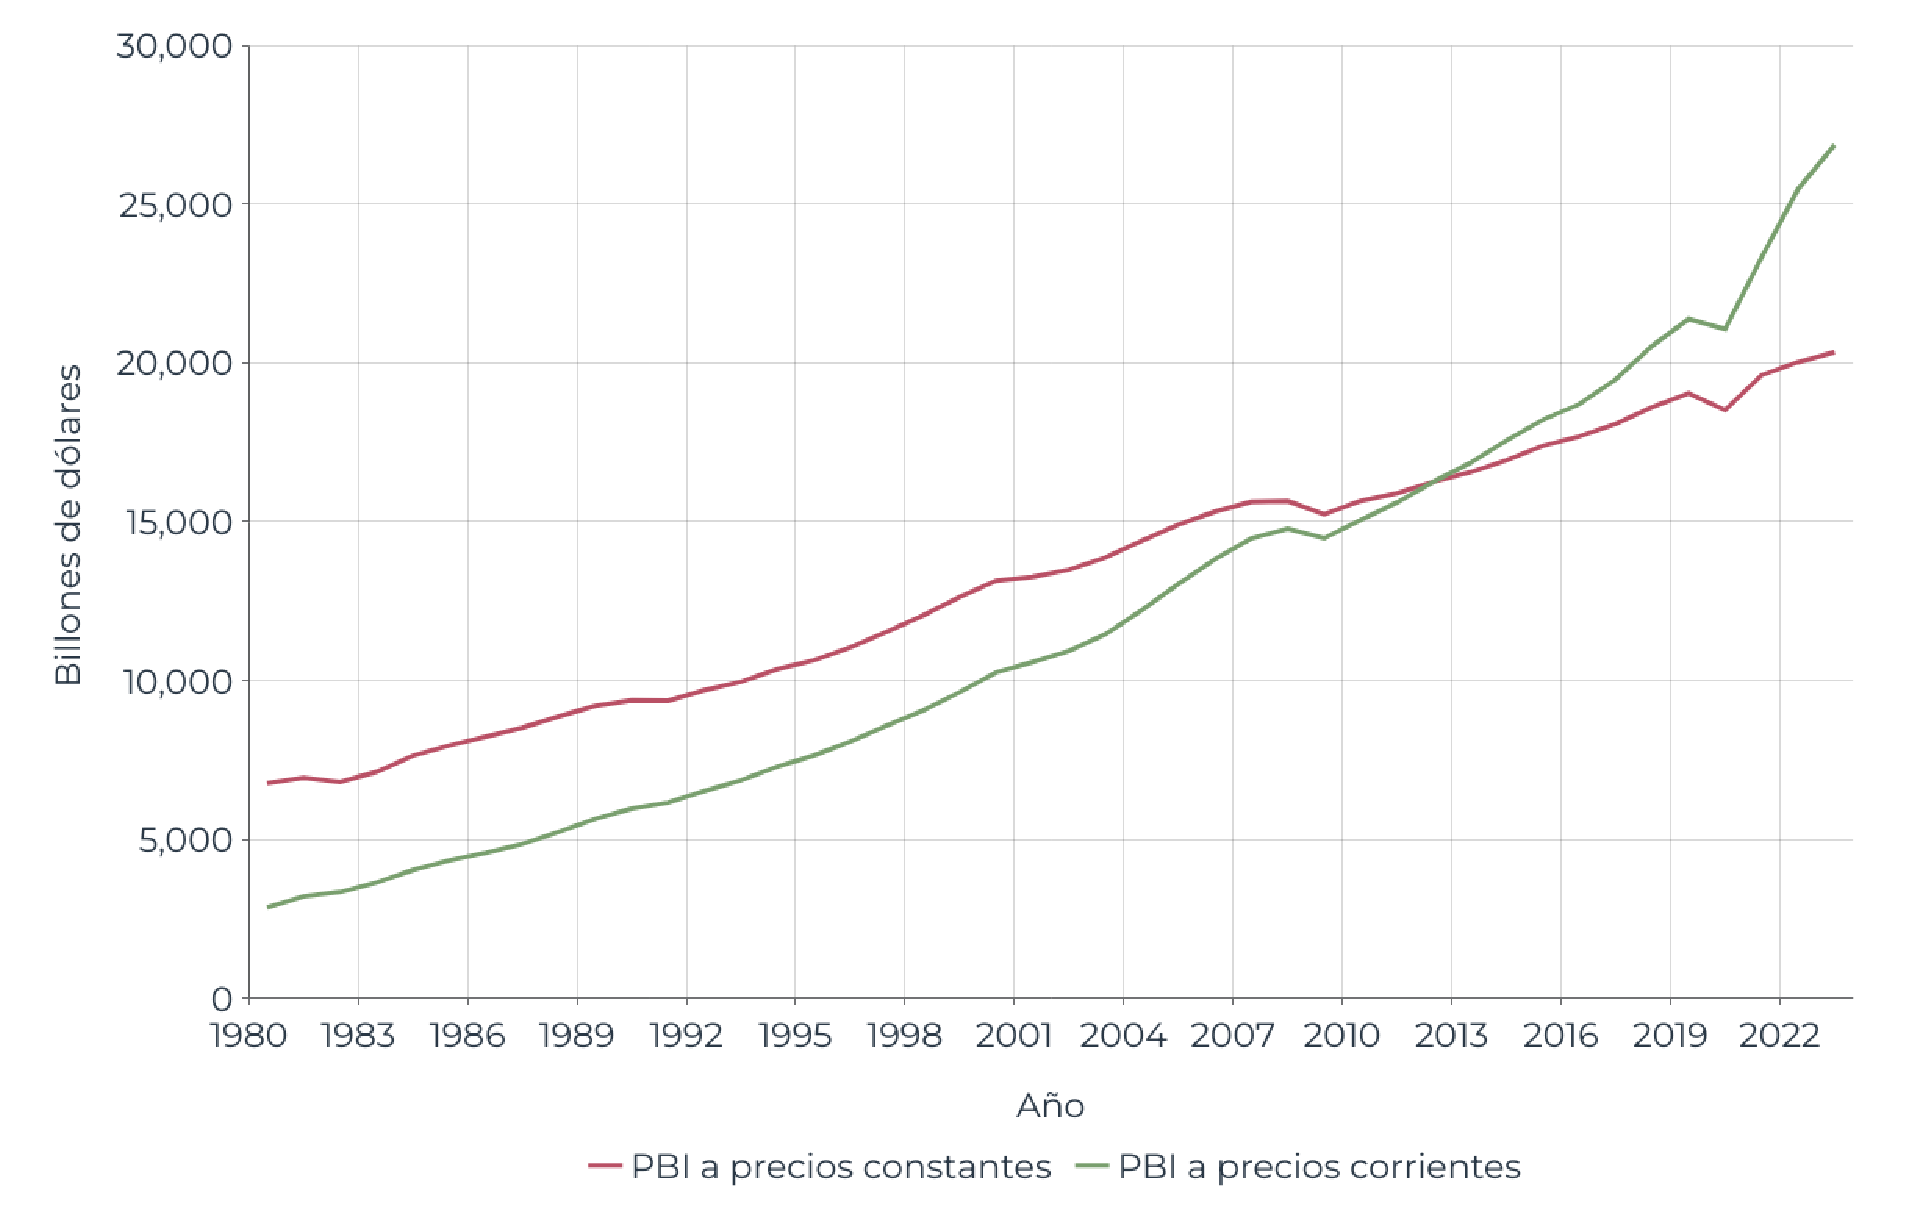
\includegraphics[width=0.9\textwidth]{Slides Principios de Economia/Figures/29.8.pdf}
\end{figure}
\end{frame}
 

\begin{frame}{PBI Nominal y real de Argentina}
    \begin{figure} [H]   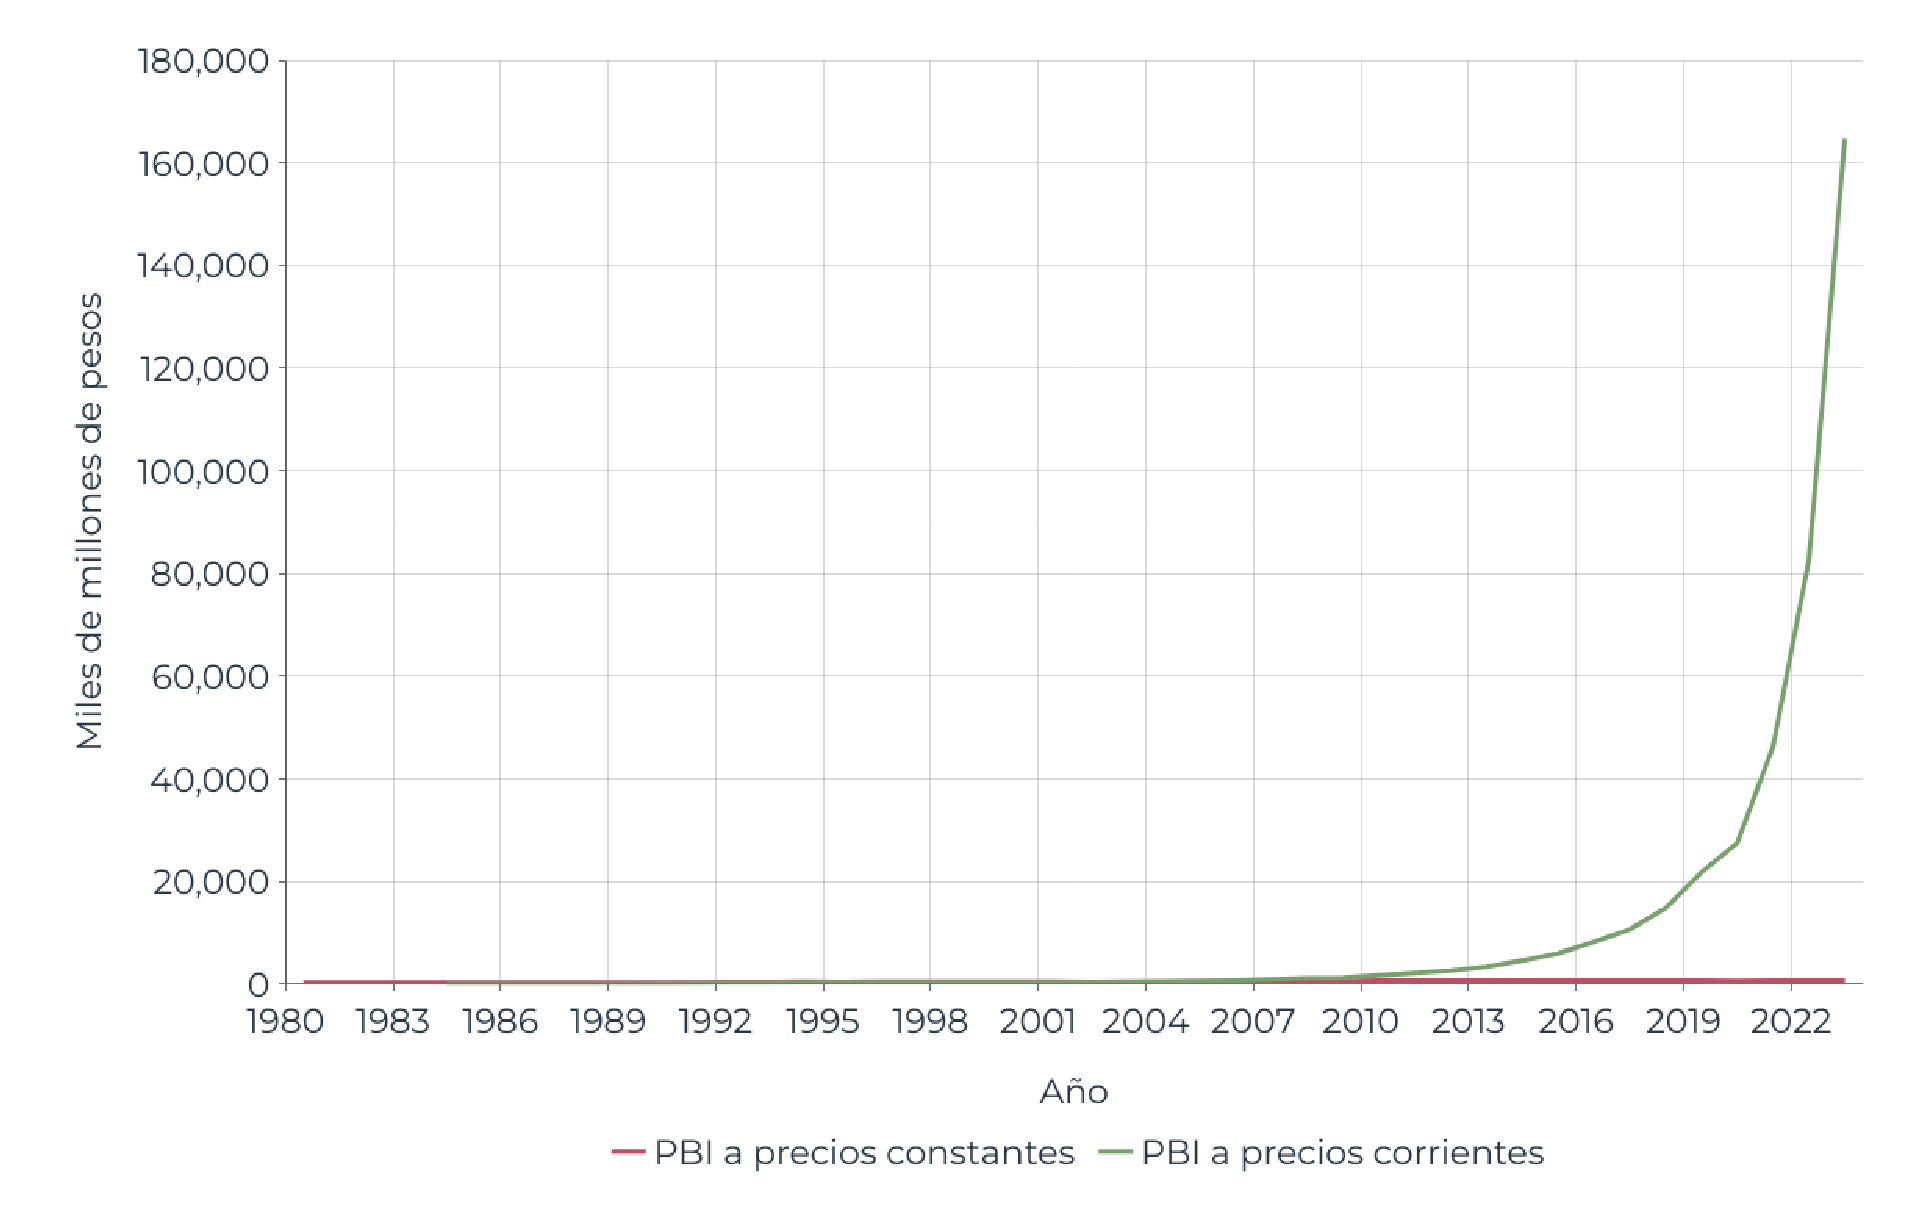
\includegraphics[width=0.9\textwidth]{Slides Principios de Economia/Figures/29.9.pdf}
\end{figure}
\end{frame}

\begin{frame}{}
\centering\huge\textbf{Desglose del PBI} 
\vspace{2mm}
\hrule
\end{frame}

\begin{frame}{Componentes y desglose del PBI}
    \begin{itemize}
    \item Haciendo referencia a los sectores que los producen (se originan en la agricultura, la minería, la industria, el comercio, el turismo, etc.) 
        \begin{itemize} \vspace{1mm}
            \item A esta referencia la llamaremos el \textit{PBI por el lado de la oferta}
        \end{itemize} \vspace{2mm}
     \item Según el uso de los bienes: vamos a segmentar el PBI según los bienes se usan para el consumo, la  inversión, el consumo público, el sector externo o la acumulación de inventarios \vspace{1mm}
     \begin{itemize}
            \item A esto lo llamaremos el \textit{PBI por el lado de la demanda}
        \end{itemize}
\end{itemize}
\end{frame}

\begin{frame}{El PBI por el lado de la oferta}

\begin{figure} [h!]
    \centering
    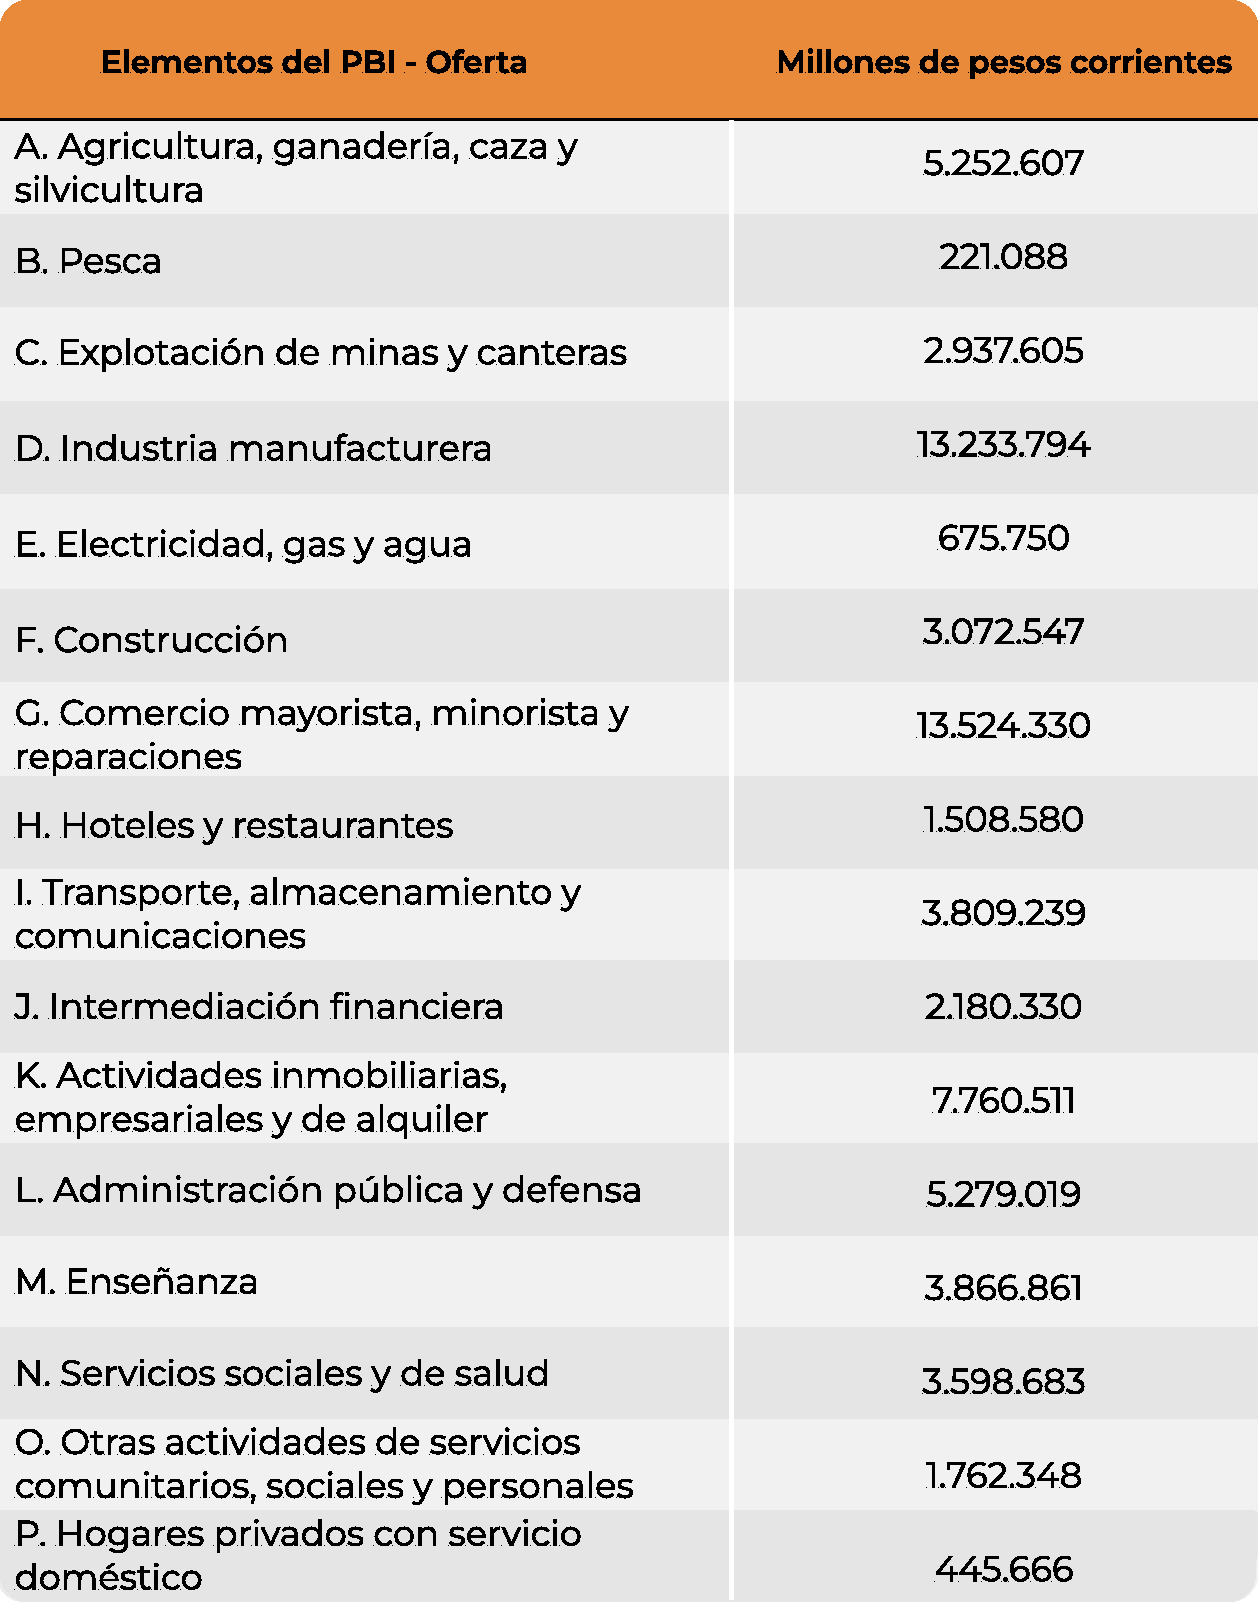
\includegraphics[width=0.5\textwidth]{Slides Principios de Economia/Figures/T 29.3.pdf}
\end{figure}

\end{frame}

\begin{frame}{El PBI por el lado de la demanda}

\begin{figure} [h!]
    \centering
    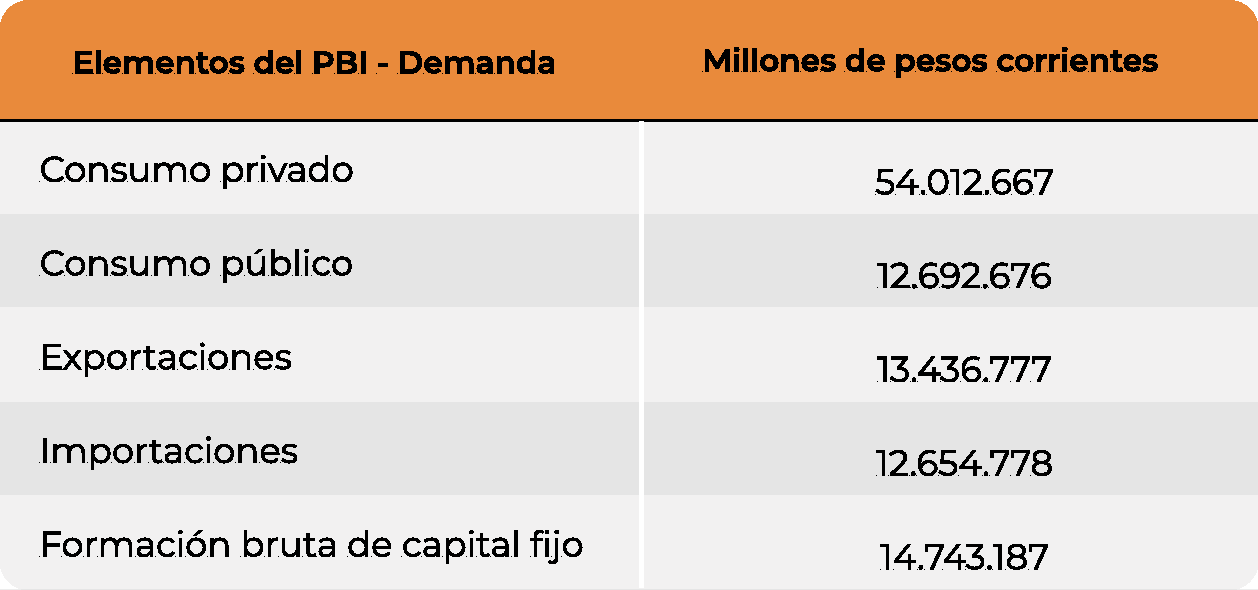
\includegraphics[width=0.9\textwidth]{Slides Principios de Economia/Figures/T 29.2.pdf}
\end{figure}

\end{frame}

\begin{frame}{El PBI por la demanda}
    
  \begin{equation}
        Y= C + I + G + X - M +  \Delta Inv.
  \end{equation}
  \begin{itemize}
  \item Esta es una ecuación muy conocida en macroeconomía
  \end{itemize}
\end{frame}

\begin{frame}{}
\centering\huge\textbf{PPP} 
\vspace{2mm}
\hrule
\end{frame}

\begin{frame}{¿Cómo se compara el PBI entre países?}
    \begin{figure} [H]   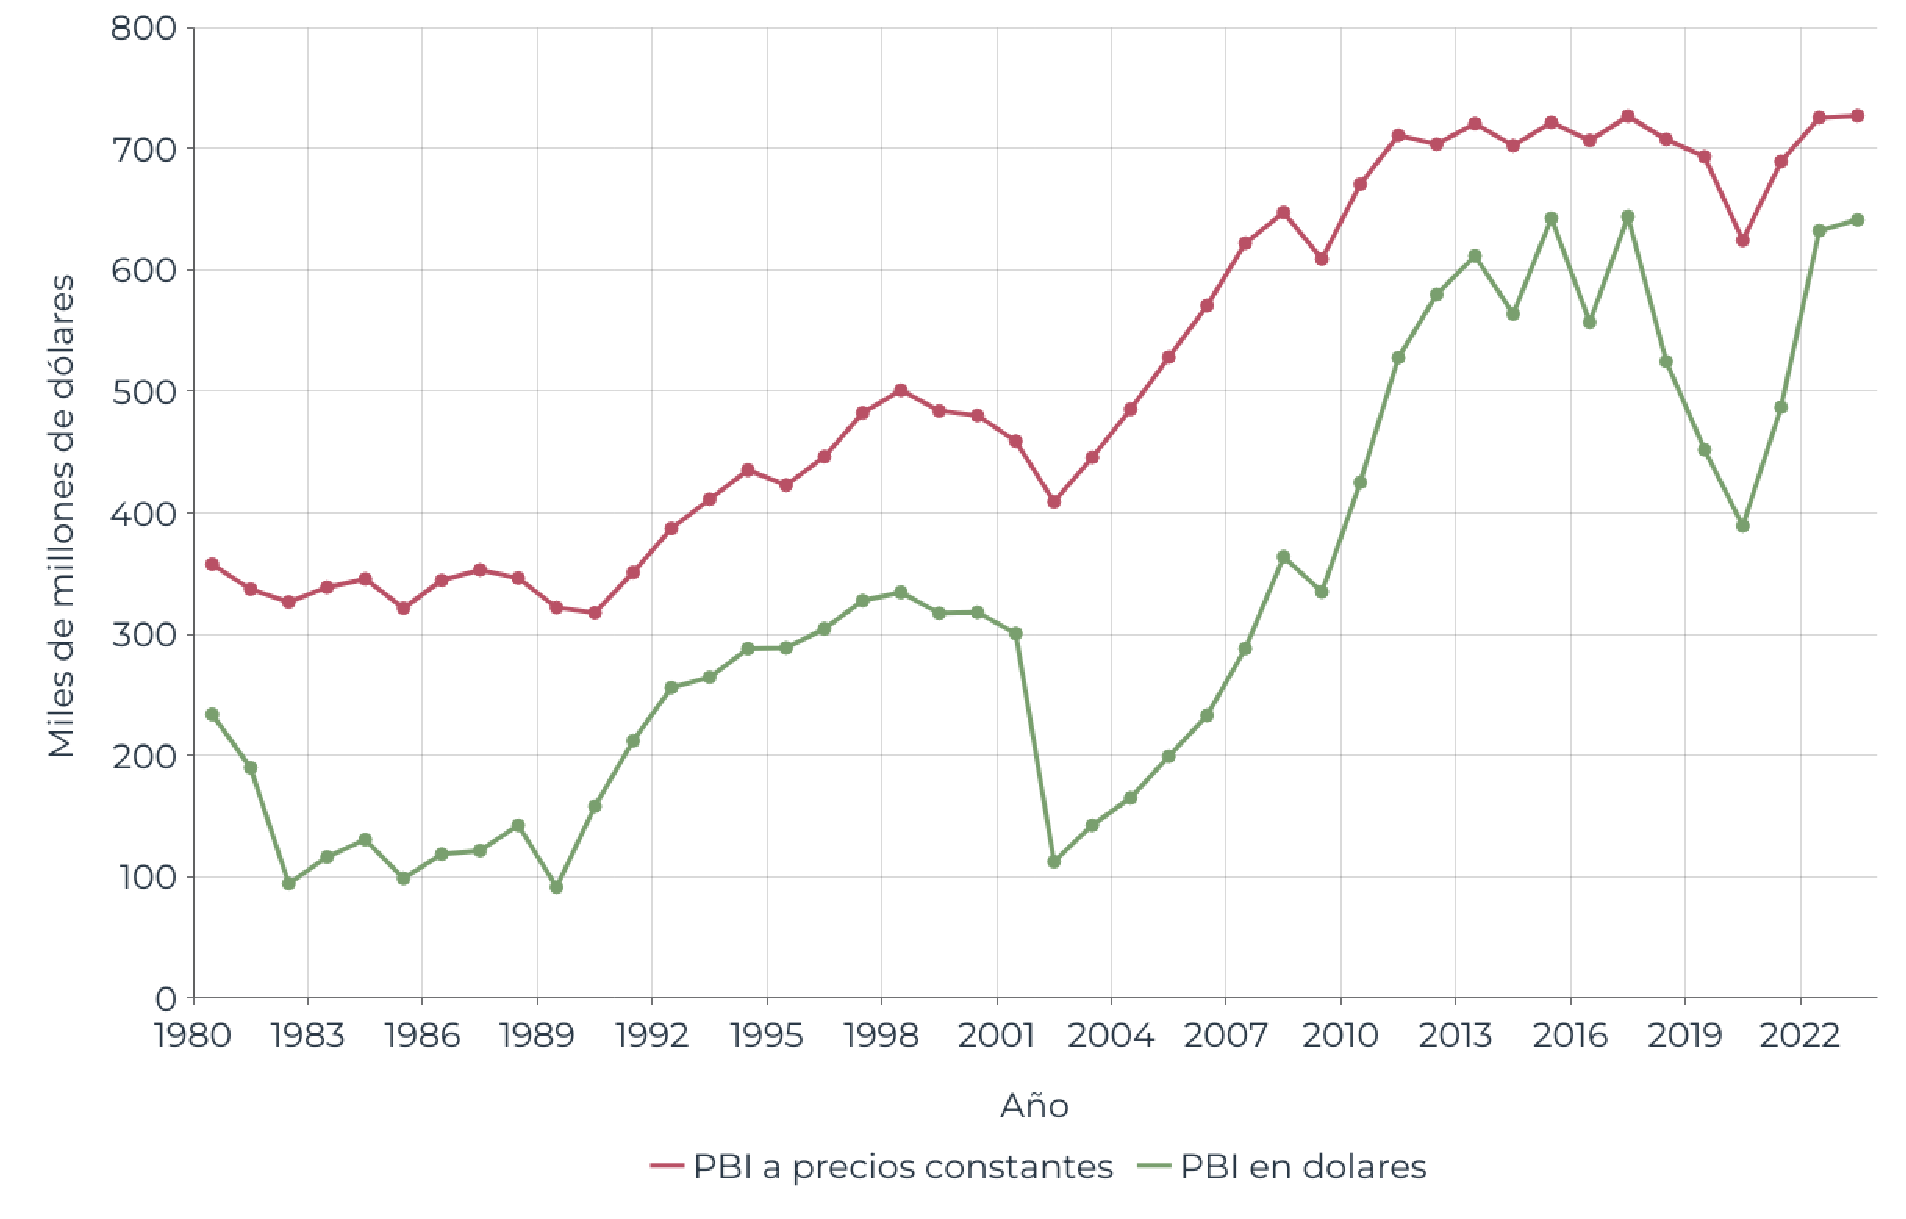
\includegraphics[width=0.9\textwidth]{Slides Principios de Economia/Figures/29.10.pdf}
\end{figure}
\end{frame}
                   
\begin{frame}{PBI en dólares y PBI en PPP}
\begin{itemize}
    \item PBI de EEUU es USD 59.041 \vspace{1mm}
    \item PBI de India es 142.073 rupias \vspace{1mm}
    \item PBI de India (en USD) es de USD 965  \vspace{1mm}
    \item Una mejor medida es el PBI de India medido en los precios de EEUU \vspace{1mm}
    \item Con ese cálculo el PBI PPP de India es de 6.461
\end{itemize}
\end{frame}

\begin{frame}{Una comparación India-China-EEUU}
   \begin{figure}[H]
\centering
    \subfigure{
\resizebox{0.42\textwidth}{!}{%
    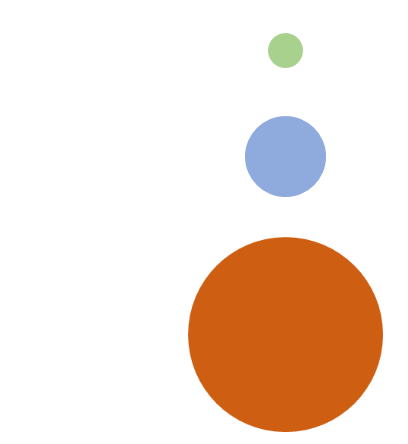
\includegraphics[width=0.9\textwidth]{Slides Principios de Economia/Figures/G4.2A.png}}}
  \hfill 
    \subfigure{
\resizebox{0.42\textwidth}{!}{%
    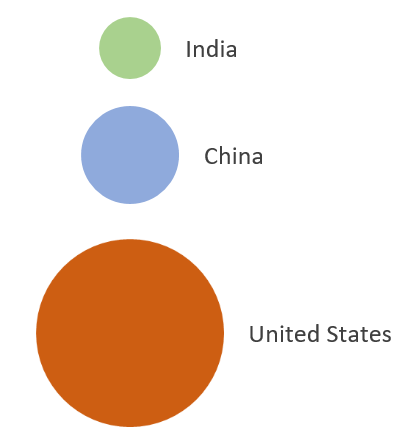
\includegraphics[width=0.9\textwidth]{Slides Principios de Economia/Figures/G4.2B.png}}}
\end{figure} 
\end{frame}

\begin{frame}{Otra comparación}
    \begin{figure} [H]   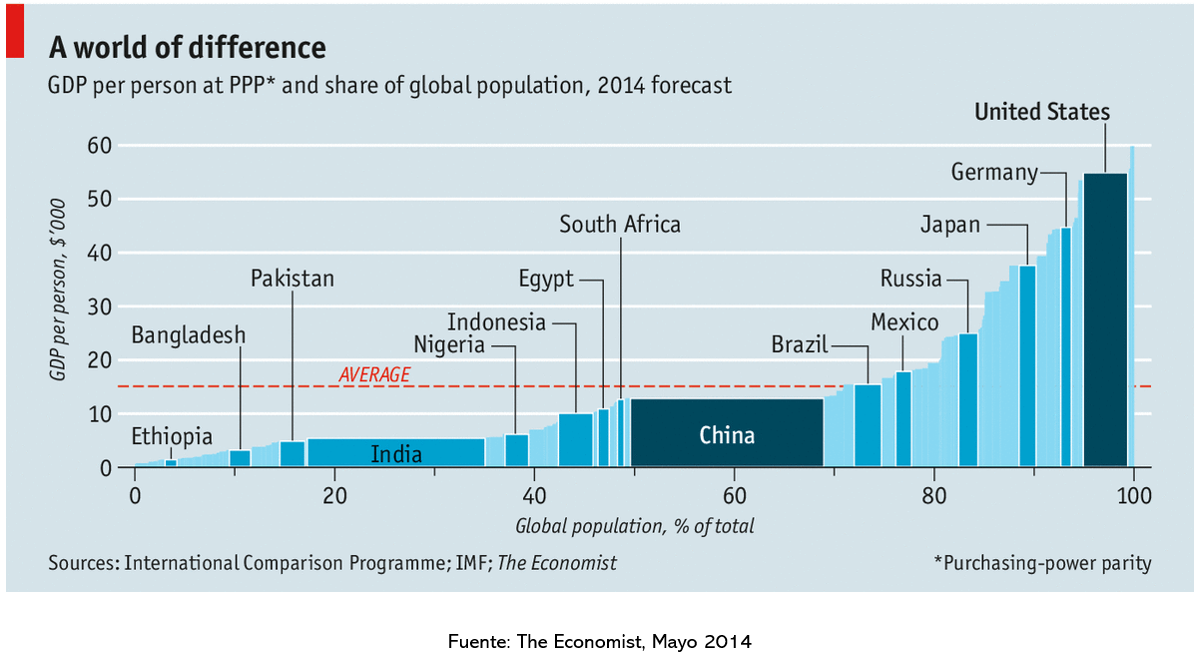
\includegraphics[scale=0.4]{Slides Principios de Economia/Figures/C16.6.png}
\caption{\textbf{¿Cómo comparamos los ingresos en el mundo?}}
\label{fig:16.6}
\end{figure}

\end{frame}


\begin{frame}{Índice de desarrollo humano}
    Las Naciones Unidas (ONU) crearon el Índice de Desarrollo Humano que está conformado por tres indicadores claves: \vspace{1mm}
\begin{itemize}
    \item Ingresos (PBI per cápita ajustado por PPP) \vspace{1mm}
    \item Longevidad (esperanza de vida al nacer) \vspace{1mm}
    \item Conocimiento (alfabetización y años de estudio).
\end{itemize} \vspace{2mm}
    Es un indicador mas amplio del bienestar que el estrictamente económico

\end{frame}


\begin{frame}{Índice de desarrollo humano 2019}
\begin{figure} [H]  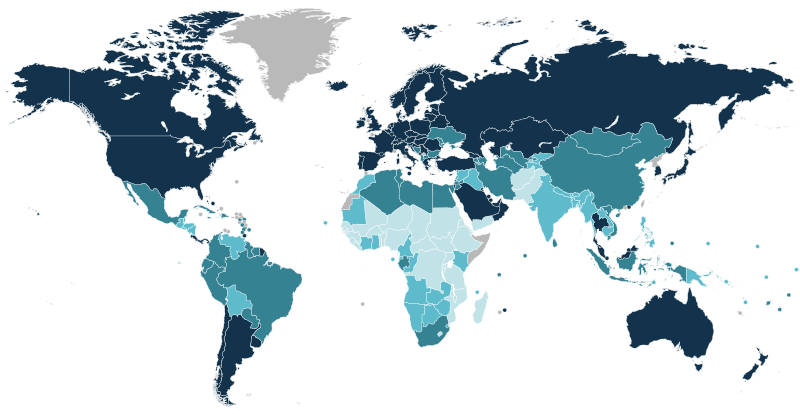
\includegraphics[scale=0.4]{Slides Principios de Economia/Figures/C16.7.png}
\end{figure}
\end{frame}

\begin{frame}{}
\centering\huge\textbf{Inflación} 
\vspace{2mm}
\hrule
\end{frame}

\begin{frame}{Midiendo la inflación}
\begin{itemize}    
    \item Típicamente para medir la inflación se elige una canasta de bienes \vspace{1mm}
    \item Definida la canasta de bienes, el nivel de precios es: 
        \begin{equation}
            P_t = p_1 q_1^c+ p_2 q_2^c...p_n q_n^c,
        \end{equation}

    \\ donde $q_i^c$ es la participación del bien $i$ en la canasta de consumo que se considera

    \item A su vez la tasa de inflación sería 

    \begin{equation}
        \pi =\frac{P_t - P_{t-1}}{P_{t-1}}= \frac{\vartriangle P}{P_{t-1}}.
    \end{equation}
\end{itemize}
\end{frame}

\begin{frame}{Midiendo la inflación}
\begin{figure} [H]  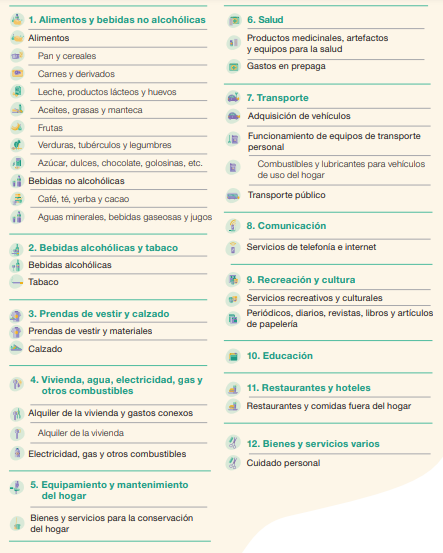
\includegraphics[scale=0.4]{Slides Principios de Economia/Figures/Canasta INDEC.png}
\end{figure}
\end{frame}

\begin{frame}{Problemas con el índice}
    \begin{itemize}
        \item Eligiendo la canasta \vspace{1mm}
        \item Ajustando por calidad \vspace{1mm}
        \item Sesgo de sustitución \vspace{1mm}
        \item Sesgo de sub-reporte \vspace{1mm}
        \item Hay distintos tipos de índices de precios (consumidor, construcción, etc.)
    \end{itemize}
\end{frame}

\begin{frame}{}
\centering\huge\textbf{Deflactor del PBI} 
\vspace{2mm}
\hrule
\end{frame}

\begin{frame}{Deflactor del PBI }
\begin{itemize}
\item ¿Existe una medida de precios del conjunto de bienes de la economía? 
\item Es el índice más agregado de los precios de toda la economía, incluyendo no solo los bienes de consumo, sino también los de inversión, exportación, etc.
\item No incluye importaciones pero si todas las exportaciones
\\ \vspace{2mm}
El deflactor del PBI es
        \begin{center}                              $PBI_{deflactor}^{\text{año i}}=\frac{PBI_{nominal}^{\text{año i}}}{PBI_{real}^{\text{año i}}} x 100$
        \end{center}
\end{itemize}
\end{frame}

\end{document}
